\chapter{Attack vectors}
\label{chp:attack-vectors}

In this chapter, we describe several methods to gain control over a program vulnerable to stack buffer overflow attacks.
In each of the sections, it is assumed that none of the measures from \cref{chp:current-defense-mechanisms} are enabled or active unless otherwise stated.
Additionally, it is assumed that an adversary has access to the executable binary which is attacked and can thus statically analyze it.

In \cref{sec:code-injection,sec:code-reuse} we present the two basic types of stack buffer overflow attacks, \crtlnameref{sec:code-injection} and \crtlnameref{sec:code-reuse}.
As their basic approaches are easily mitigated by different defense mechanisms presented in \cref{chp:current-defense-mechanisms}, the successive sections then present additional attack techniques and several possibilities on how to bypass certain security measures.

\todo{
 Differentiate between RIP and SFP overwriting? 
 If yes, in sections if applicable or in own section?
 What about overwriting data in general?
 Maybe own section at the end? Or somewhere in the middle?
}

\section{Code injection}
\label{sec:code-injection}

\Cref{subsec:ci-operating-principle} first presents what code injection is and how it works.
\Cref{subsec:ci-operating-principle} then provides information on what makes it difficult to succeed in code injection attacks and how they can be mitigated.

\subsection{Operating principle}
\label{subsec:ci-operating-principle}

Code injection is the simplest attack vector for stack buffer overflows.
As described in \cref{sec:stack-buffer-overflows}, an attacker might try to overwrite the \gls{rip}.
If this is possible, an attacker can divert control flow to any location he wants.

At such locations, the attacker can place so-called \emph{shellcode} before overflowing the vulnerable buffer.
Shellcode is the binary representation of assembly instructions compiled to the corresponding \glspl{opcode}.
Such code can be directly executed by the processor without the need of compilation (high-level programming languages like C) or translating assembly instructions with an assembler.
Shellcode can be created by compiling the desired code or assembling the desired assembly instructions into an executable file.
The executable binary shellcode can then be extracted from the resulting binary file%
	\footnote{Public databases like \href{https://www.exploit-db.com/shellcodes}{exploit-db.com} already provide lots of pre-compiled shellcode suitable for different architectures and \glspl{os}.}%
.
The name \emph{shellcode} is derived from the general attacker's goal to spawn a shell and thus execute arbitrary commands.
However, shellcode can contain any instructions and does not necessarily have to spawn a shell on the attacked system directly.

\subsubsection{Code injection into the vulnerable buffer}
\label{subsubsec:ci-into-vuln-buffer}

One possibility for an attacker to execute shellcode is to place the shellcode into the buffer which is overflown before the \gls{rip} value, as they control the buffer's contents.
The return address then has to be overwritten with the address of the buffer on the stack.
If the right address is used, the program does not return to the caller function as intended but to the position on the stack where the overwritten buffer is located.
The processor then tries to decode the data on the stack as processor instructions and thus executes the shellcode stored in the buffer.

Such an attack is very hard to achieve correctly, as the return address written onto the stack has to match the buffer's address exactly.
An offset of the return address to the buffer's address of a single byte can already render the shellcode unusable, as the instructions are decoded incorrectly by the processor.
Thus, a common technique to improve the reliability of such an exploit is to include a so-called \emph{\gls{nop} sled} into the user-controlled input which is used to overflow the vulnerable buffer on the stack.
A \gls{nop} sled consists of binary encoded \acs{nop} assembly instructions (byte \texttt{0x90} on \texttt{x86/x86\_64}).
This instruction tells the processor to do nothing during the cycle where this instruction is executed.
If a lot of such instructions are placed in front of the shellcode into the buffer, the return address does not necessarily have to point exactly to the start of the buffer or the start of the shellcode but it is sufficient to point the return address to a location somewhere in the \acs{nop} sled.
When returning into the \acs{nop} sled, the processor then executes several \gls{nop} instructions and progresses on the stack until it reaches the shellcode.

It is also possible to place the \acs{nop} sled after the shellcode on the stack instead of in front of the shellcode.
If the length of the shellcode and the \acs{nop} sled is known, a relative jump can be added to the end of the \acs{nop} sled with the negative offset for the relative jump being the combined length of the shellcode and the \acs{nop} sled.
As shown in \cref{fig:stack-overflow-nop-sled}, such a \acs{nop} sled can even extend over the overwritten return address with the help of a second relative jump in order to bypass size restrictions given by the size of the buffer.

\begin{figure}[htb]
	\centering
	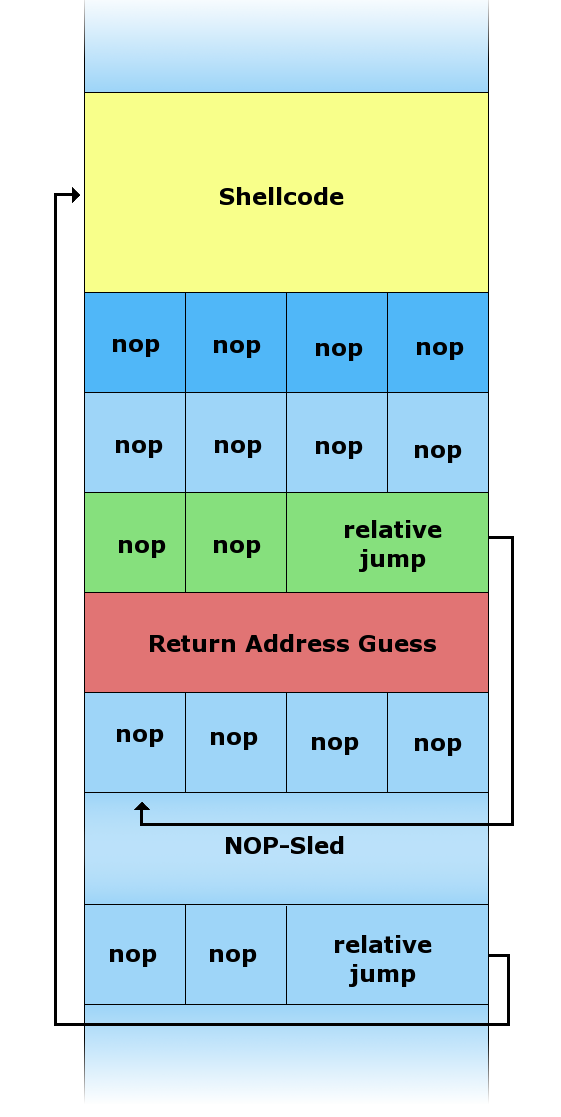
\includegraphics[width=0.3\textwidth]{figures/NopSled}
	\caption{Stack layout after a stack buffer overflow with shellcode and \acs{nop} sled \cite{Lynn2007c} (cf. \cref{fig:stack-layout})}
	\label{fig:stack-overflow-nop-sled}
\end{figure}

In general, a long \acs{nop} sled is desired by an attacker, as it becomes easier to guess an address inside of the \acs{nop} sled \cite{AlephOne1996}.

\subsubsection{Code injection via environment variables}
\label{subsubsec:ci-via-env-variable}

If it is desired to have a contiguous block of shellcode with maybe a \acs{nop} sled in front of it without the necessity of relative jumps, it might be a problem to have the exploit code fit into the vulnerable buffer before the overwritten return address, as the buffer might be too small to store the whole input.
In such cases, the actual exploit code (\acs{nop} sled and shellcode) can be put into an environment variable on the system which is being attacked if the attacker has the necessary access to the system to set environment variables.
There are slight offsets depending on the contents of other environment variables, but an environment variable generally can be found at the same address in each started process, as environment variables are loaded at the bottom of the stack \cite[731\psq]{Bryant2011}.
This allows to retrieve the location at which an environment variable will be located in the attacked process with the help of a second program (cf. \cref{lst:getenvaddress}).

Thus, it is possible to point the return address into an environment variable instead of the overflown buffer.
If the return address successfully points either directly to the shellcode or into the \acs{nop} sled inside the environment variable, the shellcode is executed exactly as in the previous case where it was put into the user-controlled overflown buffer.

A restriction of this approach is that environment variables are only mapped into the processes address space when the process is started.
Thus, shellcode cannot be injected into already running programs with the help of environment variables but only into programs started after setting the environment variable.

\subsubsection{Code injection into global variables}
\label{subsubsec:ci-via-globals}

If the shellcode is put into an environment variable, it is pretty easy to locate in memory as described above.
If this is not possible because an attacker wants to target an already active process, the shellcode has to be written onto the stack.
The difficulty of this approach is to find suitable addresses to point the \gls{rip} to when overflowing a vulnerable buffer, as stack addresses are highly volatile depending on the depth of the call stack and the functions' local variables.

If there is the possibility to place data in a global buffer before overflowing the local buffer as shown in \cref{lst:local-global-buffer}, an attacker can also put the shellcode into the global buffer and overwrite the \gls{rip} by overflowing the local buffer so that it points into the global buffer.
This greatly eases finding the target address in comparison to stack addresses, as global variables are located in the \texttt{.bss} (uninitialized global variables) or \texttt{.data} (initialized global variables) sections in an \gls{elf} executable and thus are loaded at specific memory locations as seen in \cref{lst:local-global-buffer-disassembly,fig:memory-layout}.
In the given example, the global buffer is always located at the address \texttt{0x0000000000404080}.

\lstinputlisting[language=C,float=ht,caption={C program reading data from \texttt{\acs{stdin}} into a global and a local buffer},label={lst:local-global-buffer}]{code/local-global-buffer.c}

\begin{lstlisting}[language=bash,float=ht,caption={Disassembly excerpt of the 64 bit binary compiled from the code in \cref{lst:local-global-buffer} with \texttt{gcc -o local-global-buffer local-global-buffer.c -no-pie}, retrieved with \texttt{objdump -D local-global-buffer}}, label={lst:local-global-buffer-disassembly}]
        ...

Disassembly of section .bss:

0000000000404060 <completed.7393>:
...

0000000000404080 <global_buffer>:
...
\end{lstlisting}

\subsubsection{Code injection into arbitrary buffers}
\label{subsubsec:ci-into-arbitrary-buffer}

Shellcode can also be read into any local buffer on the stack that is user-controlled before overflowing the vulnerable buffer.
However, as already mentioned \hyperref[subsubsec:ci-via-globals]{above}, it can be difficult to locate such a buffer on the stack even when using a \acs{nop} sled.

\subsection{Difficulties and countermeasures}
\label{subsec:ci-countermeasures}

Over the last 24 years since \citeauthor{AlephOne1996}'s article \citetitle{AlephOne1996} was published, several changes in processor architecture, such as the transition from 32 bit \texttt{x86} to 64 bit \texttt{x86\_64}, as well as lots of newly introduced mitigation techniques made it difficult or even impossible to inject code into a program's address space and execute such code.
On the one hand, the following measures can prevent arbitrary code execution through code injection.
On the other hand, they usually cannot prevent a \gls{dos} attack against the targeted process.
Even if it is not possible to inject code into the process's address space, a stack buffer overflow might enable an attacker to either crash the program by provoking a \gls{segfault} (cf. for example \hyperref[subsubsec:ci-data-execution-prevention]{\acl{dep}}) or shut down the process by making it detect the stack buffer overflow and exit as a reaction to the overflow (cf. for example \hyperref[subsubsec:ci-fortify-source]{\texttt{\_FORTIFY\_SOURCE}}, \hyperref[subsubsec:ci-stack-canaries]{stack canaries}).

\subsubsection{64 bit addressing}
\label{subsubsec:ci-64bit-addressing}

With the transition from \texttt{x86} to \texttt{x86\_64}, the addresses changed from a length of 32 bits / 4 bytes to 64 bits / 8 bytes.
However, the Linux kernel with the default 4-level page tables only uses 47 of the address bits for userspace virtual memory addresses and sets the upper 17 bits to zero.
With 5-level page tables, 56 bits are utilized and the upper 8 bits are set to zero \cite{Kernel2020}.

This fact implies that there is always at least one \texttt{0x00} byte in an userspace virtual memory address.
As such a \texttt{0x00} byte also marks the end of a string, an attacker might not be able to write past such a byte if the overflow occurs in a string operation function, such as \texttt{strcpy} or \texttt{gets}.
As the aforementioned processor architectures use little-endian byte addressing%
	\footnote{Least significant byte first in comparison to big-endian addressing with most significant byte first}%
, the \texttt{0x00} bytes come last and thus probably don't impose any problems when overwriting the return address, as the upper bytes are already set to \texttt{0x00} because of the original return address also being a userspace virtual memory address. 
However, usually a \gls{sfp} also has to be overwritten before even reaching the \gls{rip} (cf. \cref{fig:stack-layout}).
If the \gls{sfp} value cannot be overwritten with junk data because it is of importance later in the control flow, this might impose problems.
Because of this pointer also being a userspace virtual memory address, it also has the upper bytes set to \texttt{0x00} and can cause problems when overflowing a buffer with string based functions.

In an example as in \cref{lst:local-global-buffer}, this problem does not occur because \texttt{read} as a binary input function is used instead of string input functions.

\subsubsection{The \texttt{\_FORTIFY\_SOURCE} macro}
\label{subsubsec:ci-fortify-source}

As described in \cref{subsec:fortify-source}, the size checks conducted by setting the \texttt{\_FORTIFY\linebreak[0]\_SOURCE} value to a value higher than 0 are only activated if the value is set manually or compiler optimizations are enabled by corresponding compiler flags.
Thus, this is not a default defense measure.
However, when activated, the size checks at compile time and run time can successfully prevent stack buffer overflows and thus render a stack buffer overflow vulnerability basically unusable for code injection, as the program exits before the actual overflow even occurs.

\subsubsection{\glsentrylong{dep} (\glsentryshort{dep})}
\label{subsubsec:ci-data-execution-prevention}

Seeing that the \gls{nx} bit is used by the Linux kernel by default (cf. \cref{sec:executable-space-protection}), \gls{dep} features prevent stack contents from being executable by default.
For the stack being marked as executable, the \texttt{-z execstack} command line parameter has to be passed to \gls{gcc} explicitly.

Thus, it is not possible to make use of code injection into a process's address space on modern \glspl{os}, as the injected code is located on memory pages marked as non-executable and trying to execute code from such pages just yields a \gls{segfault}.
This not only includes a function's local stack memory but also the memory areas where environment variables are located as well as memory regions used for storing global variables.

\subsubsection{\glsentrylong{aslr} (\glsentryshort{aslr})}
\label{subsubsec:ci-aslr}

Even if user-writable memory regions are marked as executable, for example because a \gls{jit} compiler needs to store generated code, \gls{aslr} can make it extraordinarily harder for an attacker to overwrite code pointers such as the \gls{rip} or function pointers with addresses pointing to valid memory areas and especially pointing to the user-generated shellcode or into a \gls{nop} sled.

Still, enabling \gls{aslr} cannot guarantee to prevent code injection attacks.
If \gls{aslr} is enabled but the executable is not compiled as \gls{pie}, sections in the \gls{elf} binary such as \texttt{.bss} or \texttt{.data} are still located at fixed addresses and can thus be used as a target as described in the section about \crtlnameref{subsubsec:ci-via-globals}.

Even if \gls{aslr} is enabled on the system under attack and the executable was compiled as \gls{pie} beforehand, \gls{aslr} just lowers the chance of an attacker to hit the right address but does not prevent it for sure.
The stochastic approach of \gls{aslr} and other weaknesses which are further described in \cref{chp:defense-mechanism-improvements} and where bypass approaches are presented in following sections stil allow for successful code injection attacks.
\todo{Make reference more concrete than just referring to a whole chapter}

Nevertheless, the combination of \gls{dep} and \gls{aslr} in general provides a strong defense against code injection stack buffer overflow attacks by combining memory addresses that are hard to get right with non-executable memory regions.

\subsubsection{Stack canaries}
\label{subsubsec:ci-stack-canaries}

As the \gls{gcc} C compiler automatically emits code for protecting control flow information with stack canaries (cf. \cref{sec:stack-canaries}), the \gls{sfp} and \gls{rip} on the stack are protected by this security measure.
Thus, if an adversary tries to overwrite code pointers not located in the function-local data where the overflown buffer also is located, the attack fails if the stack canary value is unknown to the attacker and they thus cannot pass the canary check in a function's epilogue.

\section{Code reuse}
\label{sec:code-reuse}

In \cref{subsec:cr-ret2libc,subsec:cr-rop,subsec:cr-jop,subsec:cr-cop,subsec:cr-srop} we first present different approaches for code reuse attacks.
They all have in common that they reuse existing code in memory instead of injecting code into the attacked process's address space.
Thus, such attacks can't be prevented by marking user-controlled memory pages such as those containing the stack memory as non-executable.
Nevertheless, approaches on how to mitigate such attacks exist and are described in \cref{subsec:cr-countermeasures}.

\subsection{Return-to-libc (\glsentryshort{ret2libc})}
\label{subsec:cr-ret2libc}

After the use of the \gls{nx} bit became more and more widespread, code injection exploits based on stack buffer overflows as described \hyperref[sec:code-injection]{above} became harder and in many cases impossible to achieve.
Attackers thus had to rely on memory pages marked as executable as targets for overwritten code pointers.
Such pages contain the current program's code or code from libraries mapped into the process's address space.

As \gls{glibc} is mapped into basically every C program's address space and contains a lot of different functions, including for example \texttt{system} to execute shell commands or \texttt{execve} to replace the current process with an arbitrary other process, functions in \gls{glibc} quickly became frequent targets for overwritten function pointers.
For example, if an attacker knows the version and virtual memory address of \gls{glibc}, they can easily determine the address of a ``/bin/sh'' string and the \texttt{system} function by their offset in the \gls{glibc} \gls{elf} file and the base address.
When they then exploit a stack buffer overflow and overwrite the targeted code pointer with the address of \texttt{system} and then put the address of ``/bin/sh'' onto the stack directly after the code pointer (in accordance with the 32 bit \texttt{x86} \gls{abi} \cites[11\psq]{Lu2015}[17\psqq]{Fog2019}), \texttt{system} is executed with ``/bin/sh'' as an argument instead of the code at the original code pointer's target \cite{SolarDesigner1997}.

\Cref{fig:ret2libc} shows the stack layout after an exemplary stack buffer overflow aiming to leverage a \gls{ret2libc} exploit.
The backwards arrangement of address and string bytes is due to the little-endian representation.

\begin{figure}[htb]
	\centering
	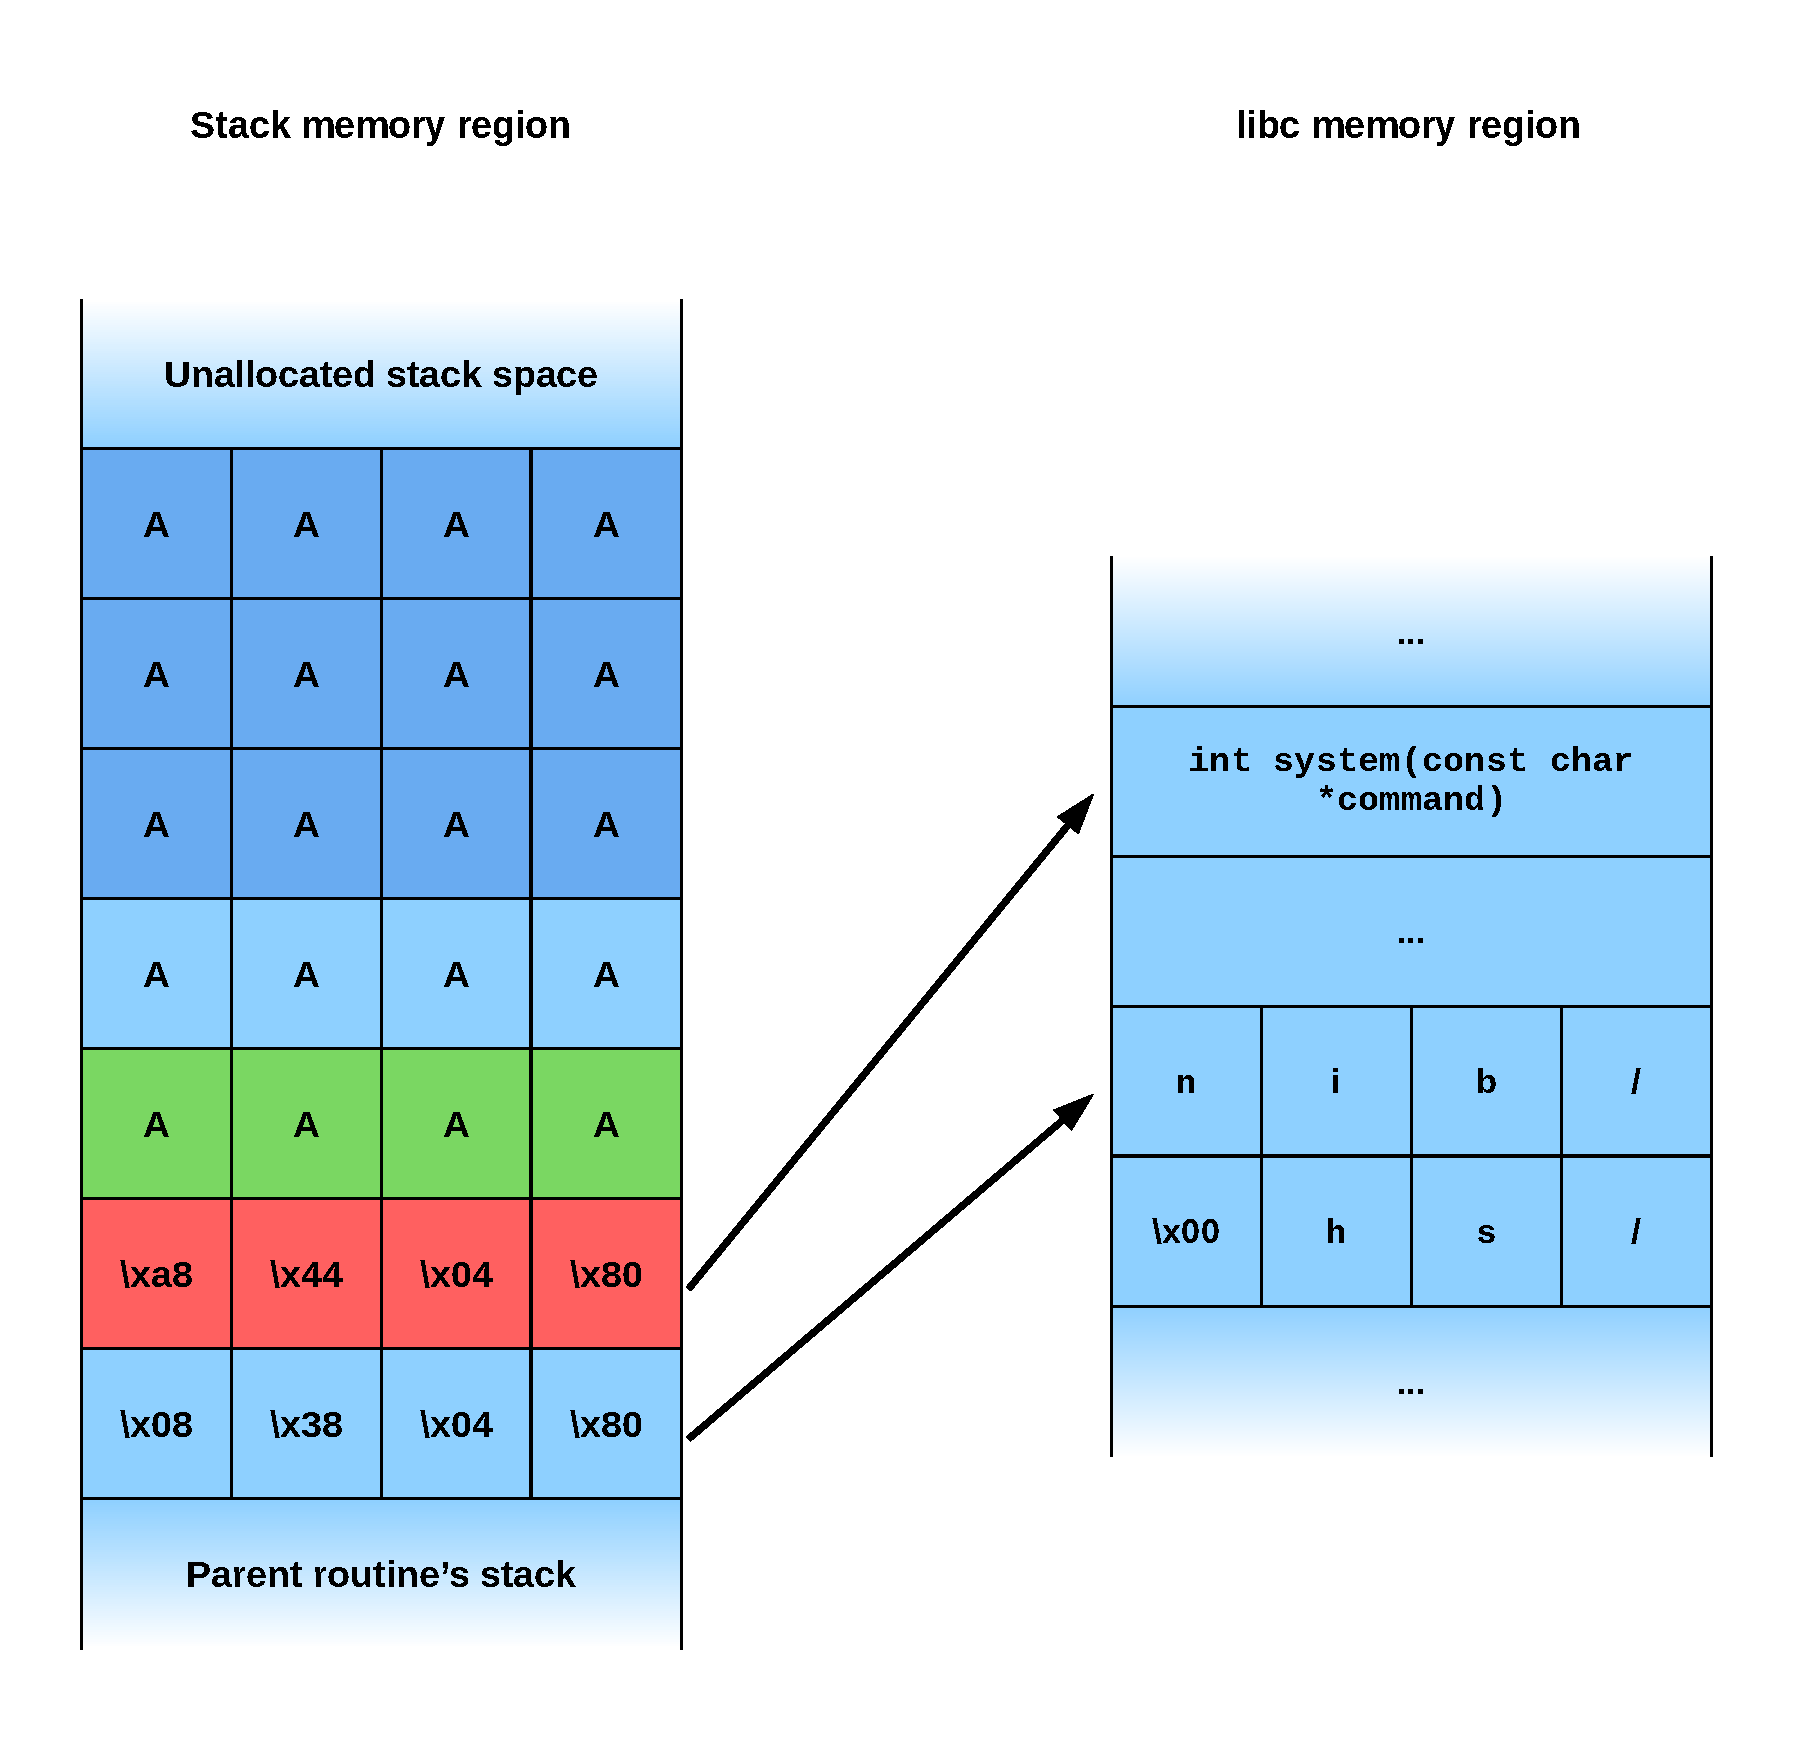
\includegraphics[width=0.8\textwidth]{figures/ret2libc}
	\caption{Stack layout after a stack buffer overflow with \acs{ret2libc} approach (own graphical representation) (cf. \cref{fig:stack-layout})}
	\label{fig:ret2libc}
\end{figure}

It is of course also possible to divert control flow to other functions in \gls{glibc} or in the executable.
A common variant of \gls{ret2libc} attacks are \gls{ret2plt} attacks where code pointers are overwritten with \gls{plt} addresses instead of the \gls{glibc} address of the targeted function.
This eases the attack, as the executable's addresses are already known before run time and thus the correct addresses in the \gls{plt} section of the executable can be easily determined.

The \gls{ret2libc} approach has a huge downside on 64 bit systems.
According to the \texttt{x86\_64} \gls{abi}, function arguments are passed in registers instead of on the stack as far as possible \cites[19\psqq]{Lu2018}[17\psqq]{Fog2019}.
Thus, it is not possible to execute arbitrary system commands or programs by overwriting code pointers with the address of \texttt{system} or \texttt{execve} without correctly setting up the necessary processor registers beforehand.


\subsection{\glsentrylong{rop} (\glsentryshort{rop})}
\label{subsec:cr-rop}

\gls{rop} is an approach to work around the \hyperref[subsec:cr-ret2libc]{aforementioned} necessity to correctly setup the processor registers in order to call specific functions on \texttt{x86\_64} machines.
Instead of exploiting a stack buffer overflow vulnerability by overwriting a code pointer (be it a function pointer in function-local data or a \gls{rip}) directly with the address of a function (e.g. \texttt{system}), the code pointer is overwritten with the address of a so-called \emph{return gadget}.
Return gadgets are short instruction chains ending in a \texttt{ret} instruction.
Such gadgets can then be chained up to execute arbitrary instructions.

Sticking with the example of an attacker trying to execute \texttt{system(``/bin/sh'')}, an attacker might try to find a gadget that pops a value from the stack into the register \texttt{rdi} and then returns by looking through the executable binary or \gls{glibc} to find byte sequences encoding such instructions that are loaded into executable memory at run time%
	\footnote{Finding such gadgets can either be done manually or automatically by using tools such as \href{https://github.com/JonathanSalwan/ROPgadget}{ROPGadget} or \href{https://github.com/sashs/Ropper}{ropper}.}%
.
The attacker would then overwrite the code pointer with the address of a \texttt{pop rdi; ret} gadget, put the address of a ``/bin/sh'' string after the gadget address so that this address is popped into \texttt{rdi} and lastly put the address of \texttt{system} after the address of the string.
This approach prepares the necessary registers (here: \texttt{rdi}) and then calls a function (here: \texttt{system}) with the attacker-controlled parameters.

Gadgets can be chained up by putting several gadget addresses one after the other onto the stack so that the \texttt{ret} instruction of a gadget automatically returns to the next gadget.
Because of this behavior, arbitrary code execution is possible as long as an attacker can find binary encodings of the necessary assembly instructions in executable memory pages of the process's address space.

\subsection{\glsentrylong{jop} (\glsentryshort{jop})}
\label{subsec:cr-jop}

\gls{jop} is similar to \gls{rop} in that they both use short gadgets which can be chained up to achieve arbitrary code execution.
The main difference, however, is that \gls{jop} is not based on gadgets ending in a \texttt{ret} instruction but in gadgets ending in an indirect \texttt{jmp} instruction.
Indirect jumps are not based on fixed addresses generated by the compiler and output into the executable binary.
Instead, their target is dynamically calculated at run time and taken from the register or memory location specified in the instruction's operand \cite[3-517\psqq]{IntelCorporation2020}.

Because \gls{rop} gadgets have bi-directional control flow (handing the control to the gadget, gadget returning back control based on the stack contents), they are easy to set up and can easily be chained based on the addresses and data put onto the stack by an attacker.
\gls{jop} gadgets on the other side inhibit uni-directional control flow by branching without regard to any following stack contents.
This behavior implies the necessity that either each gadget somehow loads the address of the next gadget in a register so that the indirect jump at the end of the gadget jumps to the next gadget or that the register's contents are updated between executing two consecutive gadgets.


\subsubsection{\glsentryshort{jop} based on dispatcher gadgets}
\label{subsubsec:cr-jop-dispatcher}

\citeauthor{Bletsch2011} propose an approach based on a dispatch table where they differentiate between \emph{functional} and \emph{dispatcher} gadgets \cite{Bletsch2011}.
The former are gadgets which contain the actual code an attacker might want to run, the latter are gadgets which are responsible for chaining up the functional gadgets so that the desired result can be achieved.
The idea is that an adversary injects a dispatch table into the program's memory which can be located at arbitrary memory (on the stack, on the heap, in global variables or anywhere else).
At the beginning of the exploit, the dispatch table address is loaded into a register and the dispatcher gadget address into a second register.
The dispatcher gadget operates on the dispatch table register and advances the address so that whenever the dispatcher gadget is executed, the dispatch table register points to the next table entry afterwards.
The table itself can be implemented for example as a consecutive array of addresses or a linked list, depending on the dispatcher gadget used.
The table entries then are the addresses of the functional gadgets which use the register containing the dispatcher gadget address as the register for the indirect jump at the end of the gadget.
This way, the dispatch table register acts as a virtual program counter that is advanced to the next gadget after each functional gadget when said gadget jumps back to the dispatcher gadget \cite{Bletsch2011}.
A simple example for such a control flow is shown in \cref{fig:jop-dispatcher}.

\begin{figure}[htb]
	\centering
	\begin{subfigure}[t]{0.8\textwidth}
		\centering
		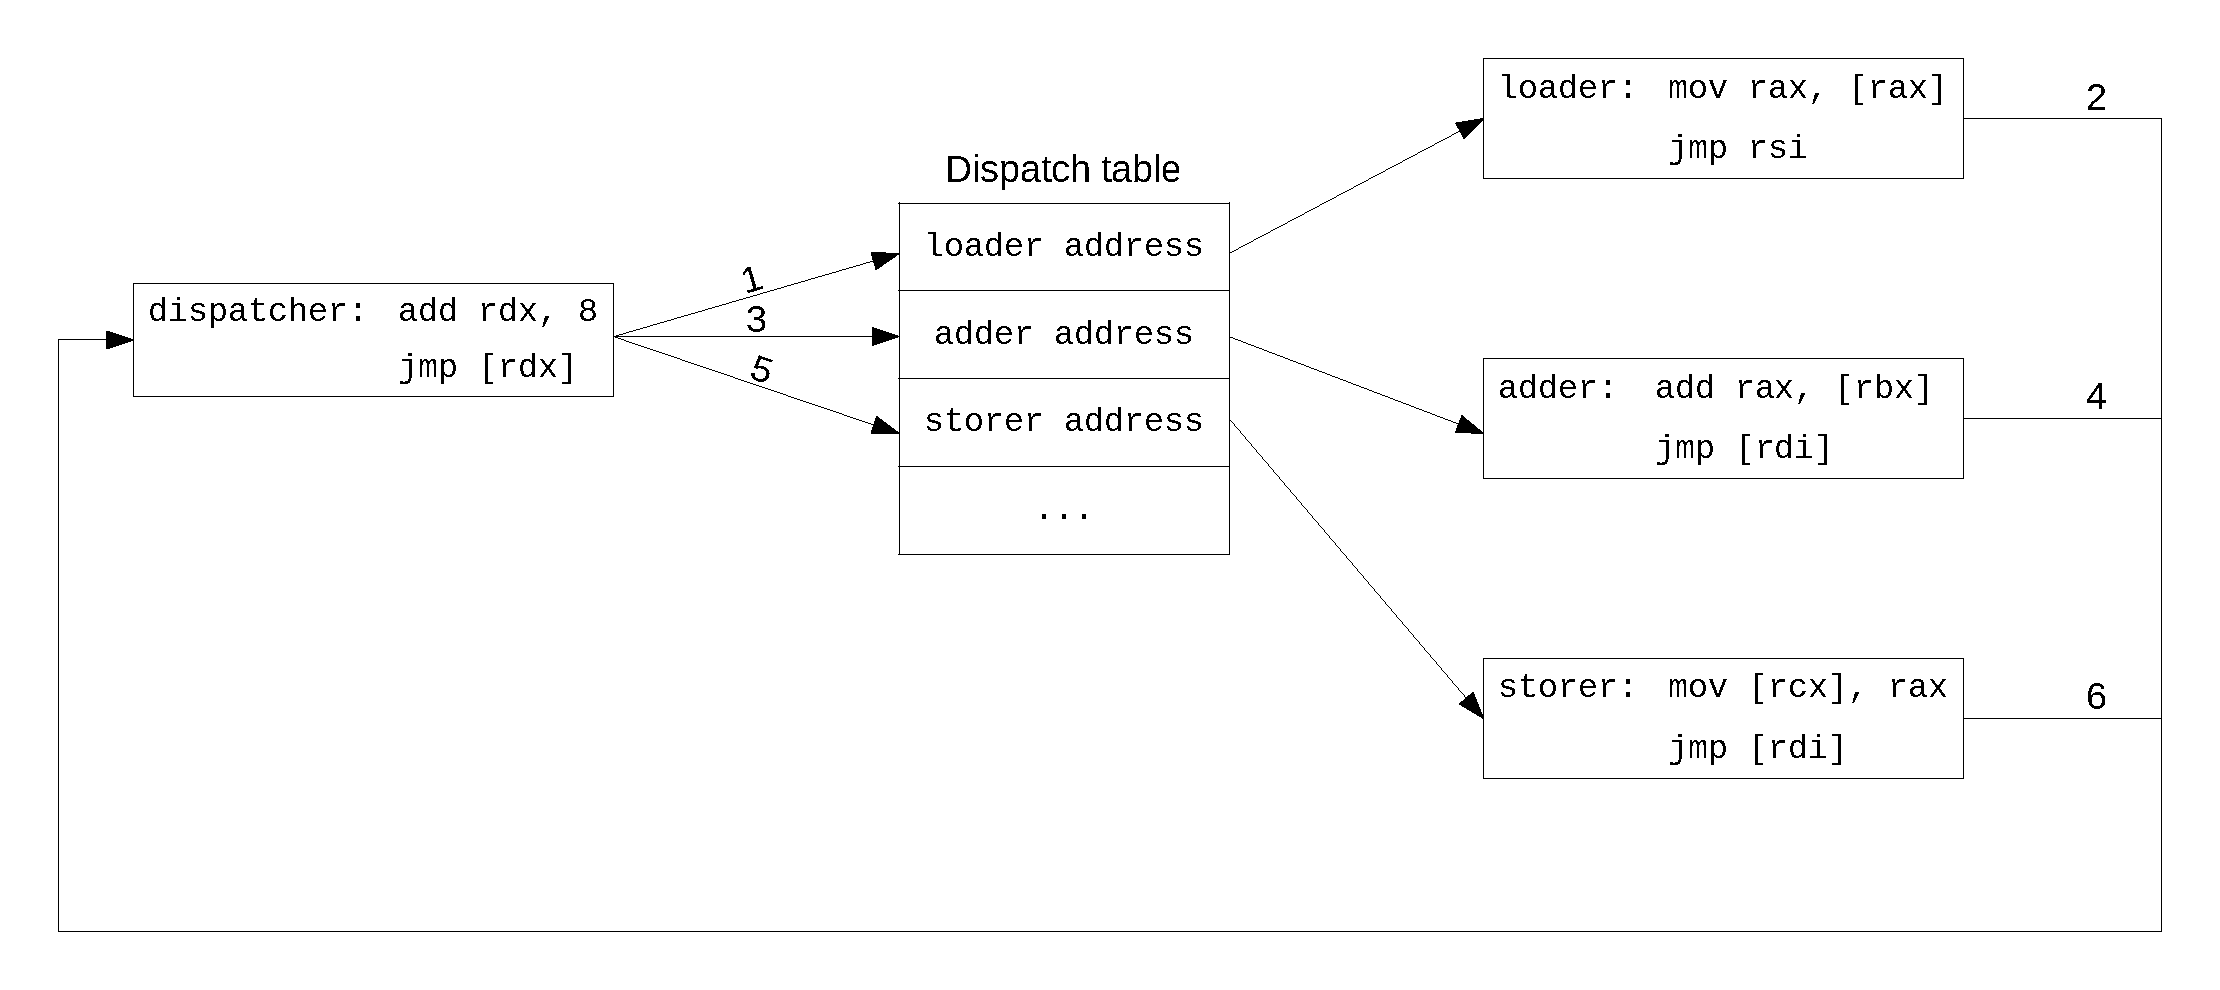
\includegraphics[width=\textwidth]{figures/jop-dispatcher}
		\caption{Exemplary \acs{jop} control flow with a dispatcher gadget (own graphical representation based on figure 3 from \cite{Bletsch2011})}
		\label{fig:jop-dispatcher}
		\vspace*{1em}
	\end{subfigure}
	\begin{subfigure}[t]{0.8\textwidth}
		\centering
		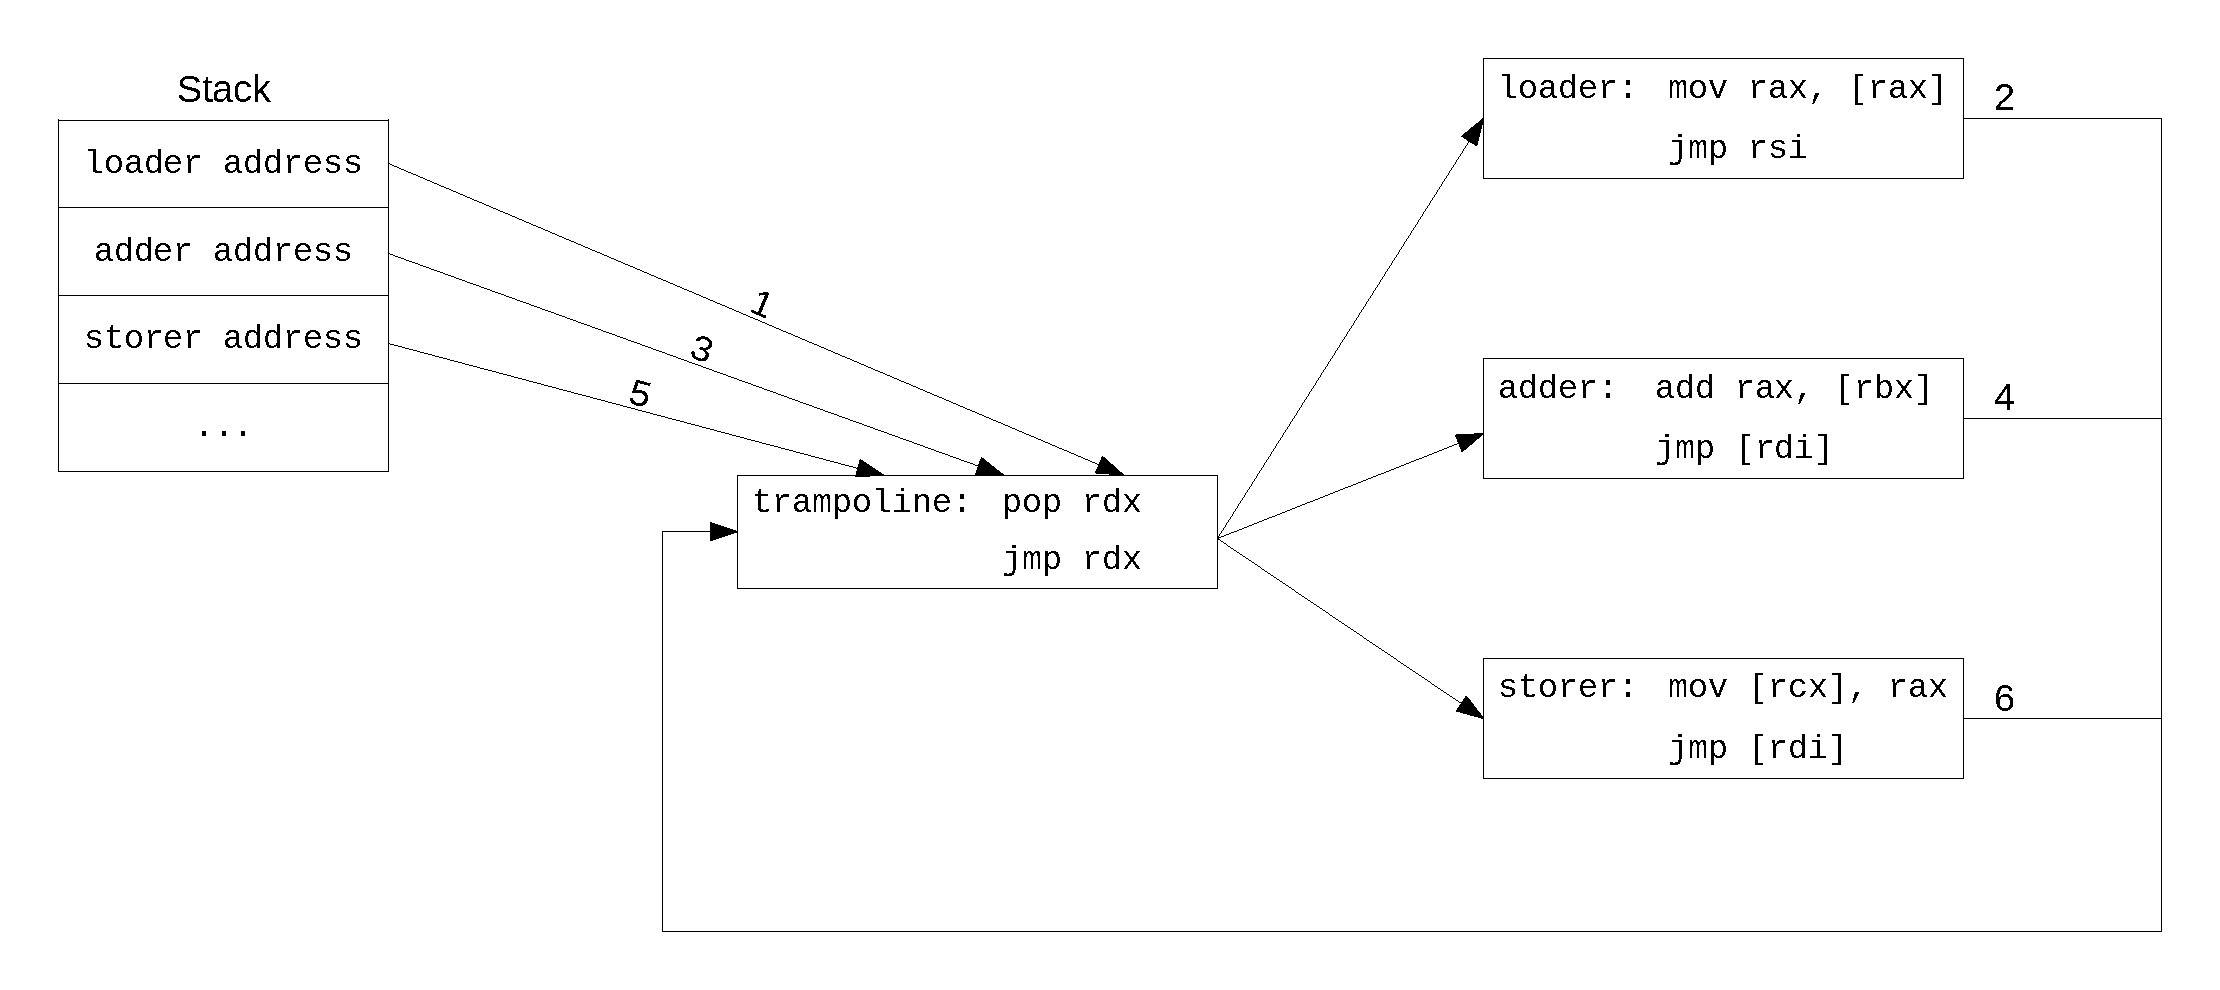
\includegraphics[width=\textwidth]{figures/jop-trampoline}
		\caption{Examplary \acs{jop} control flow with a trampoline gadget (own graphical representation based on figure 1 from \cite{Checkoway2010})}
		\label{fig:jop-trampoline}
	\end{subfigure}
	\caption{Control flow of dispatcher and trampoline based \acs{jop} exploits. Note the difference between indirect and direct jump in the dispatcher and trampoline gadget.}
	\label{fig:jump-oriented-programming}
\end{figure}

This approach has several advantages over the \gls{rop} approach:
Firstly, it does not rely on stack contents written after the overwritten code pointer.
Thus, if for example there is not enough space after the code pointer to be overwritten to put all the \gls{rop} gadgets' addresses but enough space before the code pointer to put a dispatch table, the \gls{jop} approach can still work whereas the \gls{rop} approach is blocked by its memory prerequisites.
Secondly, measures implemented to detect \gls{rop} exploits observe behavior like a high frequency of \texttt{ret} instructions which can be bypassed by \gls{jop} exploits which do not rely on that instruction \cite{Bletsch2011}.

On the other hand, a \gls{jop} exploit is more difficult to implement as it doesn't suffice to put gadget addresses onto the stack but it is also necessary to account for side-effects when a gadget manipulates one of the registers containing the dispatch table address or the dispatcher gadget address.
Therefore, it might be necessary to sometimes insert gadgets which do not contribute to the desired functionality but which are just necessary to compensate for side-effects of gadgets that interrupt the \gls{jop} chain \cite{Bletsch2011}.

\subsubsection{\glsentryshort{jop} based on trampoline gadgets}
\label{subsubsec:cr-jop-trampoline}

\citeauthor{Checkoway2010} propose an approach based on \emph{trampoline} gadgets instead of dispatcher gadgets.
Where \citeauthor{Bletsch2011} use a dispatcher gadget to manipulate a dispatch table pointer so that the indirect jump at the end of the gadget continues with the next desired functional gadget, \citeauthor{Checkoway2010} do not just modify the pointer to the next gadget but completely replace it in their trampoline gadget.
The overall idea is to include such a trampoline gadget in between functional gadgets in order to retrieve the next functional gadget address from the stack and jump to that gadget as shown in \cref{fig:jop-trampoline}.
The basic approach is thus very similar to the dispatcher gadget approach with the slight difference that the trampoline gadget based approach is relying on the stack contents similar to a \gls{rop} exploit, as it mixes gadget addresses and data on the stack just like a \gls{rop} exploit.
It thus also uses the stack pointer as a virtual program counter instead of a specified register as it is the case when using dispatcher gadgets.
\citeauthor{Checkoway2010} because of those similarities refer to their attack as ``return-oriented programming \textit{without using return instructions}'' \cite{Checkoway2010}.

Similar to the \hyperref[subsubsec:cr-jop-dispatcher]{dispatcher gadget approach}, the trampoline gadget approach can bypass \gls{rop} protections based on detecting a high frequency of \texttt{ret} instructions or a violation of the stack's \gls{lifo} principle \cite{Checkoway2010}.

\subsection{\glsentrylong{cop} (\glsentryshort{cop})}
\label{subsec:cr-cop}

A \texttt{call} instruction on \texttt{x86\_64} behaves basically like a \texttt{push rip; jmp} instruction.
It pushes the current \texttt{rip} register contents which contains the address of the next instruction onto the stack and then branches to the provided target \cite[3-122\psqq]{IntelCorporation2020}.
\todo{Page numbers as in the document, but they include hyphens because the page numbers are reset for every chapter... Not ideal, looks like a page range here}
Because of this behavior, \citeauthor{Bletsch2011} already state that \texttt{call} instructions can be used for \gls{jop} instead of \texttt{jmp} instructions as long as the exploit doesn't rely on the stack or the side-effect of pushing the return address onto the stack is compensated for by the gadgets \cite{Bletsch2011}.

\citeauthor{Sadeghi2018} further developed this idea into so-called \gls{cop} where only \texttt{call} instructions are used for chaining the gadgets.
Because of the side effect of pushing data onto the stack, they conclude that classical \gls{jop} exploits using trampoline or dispatcher gadgets do not work with purely \texttt{call}-ending gadgets.
To overcome this problem, they propose \emph{strong trampoline} and \emph{intra stack pivot} gadgets.

Strong trampoline gadgets are very similar to the trampoline gadgets described in \cref{subsubsec:cr-jop-trampoline} with the difference that they not only pop the target gadget address from the stack but ideally also two other values beforehand.
This is necessary because the previous trampoline gadget as well as the functional gadget between the two trampoline gadgets each pushed a return address onto the stack when executing their \texttt{call} instruction.
A strong trampoline gadget thus has to account for those addresses and remove them from the stack before retrieving the next functional gadget address (cf. \cref{tab:trampoline-gadgets}) \cite{Sadeghi2018}.

 \begin{table}[ht]
	\centering
	\caption{Comparison between exemplary trampoline gadget as in \cite{Checkoway2010} and strong trampoline gadget as in \cite{Sadeghi2018}}
	\makebox[\textwidth][c]{ % command is necessary in order to center the table correctly
		\bgroup
		\def\arraystretch{1.1} % changes vertical spacing so that the table looks better
		\begin{tabular}{|l|l|}
			\hline
			Trampoline gadget		& Strong trampoline gadget		\\
			\hline
			\texttt{pop rdx}		& \texttt{pop rax}				\\
			\texttt{jmp rdx}		& \texttt{pop rbx}				\\
									& \texttt{pop rdx}				\\
									& \texttt{call rdx}				\\
			\hline
		\end{tabular}
		\egroup
	}
	\label{tab:trampoline-gadgets}
\end{table}

Intra stack pivot gadgets are gadgets that manipulate the stack pointer in the \texttt{rsp} register by adding to its value \cite{Sadeghi2018}.
Pushing onto the stack advances the stack pointer by the size of the operand and then stores the value of the operand on top of the stack \cite[4-513\psq]{IntelCorporation2020}.
As we are looking at a \texttt{x86\_64} system and the stack is growing downwards in the address space, advancing the stack pointer is equivalent to subtracting 8 from the stack pointer.
Thus, the intra stack pivot gadget has to add to the stack pointer a multiple of 8 in order to dismiss the return addresses pushed onto the stack by previous \gls{cop} gadgets.
Such gadgets are useful if no strong trampoline gadgets can be found in the process's address space (i.e. in the executable binary or the binaries of the linked libraries) or for compensating stack manipulation by \texttt{push} instructions and instructions with side-effects similar to \texttt{push} instructions in general.

Using strong trampoline gadgets and intra stack pivot gadgets, attacks similar to \gls{jop} attacks based on trampoline or dispatcher gadgets can be launched purely based on gadgets ending with \texttt{call} instructions instead of \texttt{jmp} instructions \cite{Sadeghi2018}.

\subsection{\glsentrylong{srop} (\glsentryshort{srop})}
\label{subsec:cr-srop}

In addition to the previous code reuse approaches which were strongly based on chaining gadgets to manipulate the \acs{cpu} context, \citeauthor{Bosman2014} propose their \gls{srop} approach based on the signal handling behavior of UNIX-based and UNIX-like systems and as such also Linux.
When a process has a pending signal, it stores the current \acs{cpu} context including register contents, flags, etc. on the stack as soon as it transitions back to user-mode, for example by returning from a \gls{syscall} (kernel mode) or being rescheduled onto a \acs{cpu}.
Afterwards, the signal handler corresponding to the received signal is run.
When this signal handler returns, a \texttt{sigreturn} \gls{syscall} is issued which restores the process's \acs{cpu} context from the stack in order to continue execution just as the process was supposed to \cite{Bosman2014,Kerrisk2020a}.

If an adversary can exploit a stack buffer overflow vulnerability by controlling the contents of the \texttt{rax} register to set the \gls{syscall} number to 15 \cite[\texttt{arch/x86/entry/\linebreak[0]syscalls/syscall\_64.tbl}]{LKD2020} and then issue a \gls{syscall}, the contents of the stack at the current stack pointer location are interpreted as a \acs{cpu} context and the context is restored.
The adversary thus then completely controls the system behavior with a single \gls{syscall} if they set up a \texttt{sigreturn} frame on the stack beforehand, as they control all of the processor registers including the stack pointer or the instruction pointer as well as flags and other context information.

This approach is classified as a code reuse attack because it needs a gadget invoking a \gls{syscall} to trigger the \texttt{sigreturn} behavior.
The \gls{srop} approach facilitates code reuse exploits in comparison to standard code reuse attacks based on gadget chaining, as no gadgets to specifically setup the registers (apart from \texttt{rax} for the first \gls{syscall}) are needed \cite{Bosman2014}.

\subsection{Difficulties and countermeasures}
\label{subsec:cr-countermeasures}

In general, the same difficulties and countermeasures against code reuse exploits apply as for code injection attacks (cf. \cref{subsec:ci-countermeasures}).
However, some distinctions have to be made.

\subsubsection{\glsentrylong{aslr} (\glsentryshort{aslr})}
\label{subsubsec:cr-aslr}

With code injection techniques, \gls{aslr} is a huge hindering, as the stack base address and thus the address of the environment variable or the stack buffer containing shellcode changes with each process instantiation.

For code reuse attacks, \gls{aslr} only poses a problem if the executable is compiled as \gls{pie}.
If not, the addresses of binary instructions or bytes possibly interpreted as valid instructions inside the executable binary are fixed and thus the virtual memory address at which they are loaded at run time is already known beforehand.
Even though the memory base addresses of any linked libraries are still unknown and their contents thus cannot easily be taken into consideration for \gls{rop}, \gls{jop} or \gls{cop} gadgets, the actual executable may provide enough gadgets for successful attacks if it is big enough or if libraries are statically linked into it instead of dynamically loaded at run time.
If not looking at gadget-based exploits but simple function calls as described for \gls{ret2libc} or \gls{ret2plt} attacks, the \texttt{.plt} section of the executable and thus the \gls{plt} is also at a fixed position if not compiled as \gls{pie}.
Thus, \gls{ret2plt} attacks can still be leveraged like without \gls{aslr}.

If the executable is compiled as \gls{pie}, \gls{aslr} provides the same protection as against code injection attacks, as no gadget addresses can be easily determined.

\subsubsection{\glsentrylong{dep} (\glsentryshort{dep})}
\label{subsubsec:cr-dep}

The main motivation behind code reuse attacks in comparison to code injection attacks as described in \cref{sec:code-injection} is that they cannot be prevented by simple \gls{dep} measures such as the use of the \gls{nx} bit or \gls{wxorx} policies.
As they do not insert code into memory pages marked as non-executable but only depend on memory pages already marked as executable because the latter contain library or program code, code reuse exploits are immune against \gls{dep} measures and have to be countered with other security measures.

\section{\glsentryshort{got} hijacking}
\label{sec:got-hijacking}

As mentioned in \cref{sec:relro} concerning the \gls{relro} security measure, \gls{got} entries without protection through \gls{relro} and located right after the user-controlled data sections in memory could be overwritten by an attacker exploiting a buffer overflow vulnerability with a buffer located in said data sections (\texttt{.bss} or \texttt{.data}).
As this paper is referring specifically to stack based buffer overflows, such attacks are out of scope and will not be analyzed further.
However, stack buffer overflow vulnerabilities can still allow an adversary to divert control flow by precisely overwriting \gls{got} entries as presented in the rest of this section.
For this purpose it is assumed that \gls{dep} is enabled and it is thus not possible for an attacker to just put shellcode onto the stack and execute that shellcode.
Additionally, \gls{aslr} and stack canaries are enabled.
For the former, the restriction applies that the attacked program is not compiled as \gls{pie} and that parts of the process's address space are thus located at predictable addresses.

\subsection{Operating principle}
\label{subsec:got-operating-principle}

As stack canaries are present in an assumed execution of such a program with a stack buffer overflow vulnerability, it is not possible to leverage powerful code reuse attacks such as \gls{rop} by overwriting the return address without somehow bypassing the stack canary check, for example by leaking the stack canary beforehand.
In addition, with \gls{aslr} enabled, it is difficult to successfully launch a \gls{ret2libc} attack or reuse library code for \gls{rop}, \gls{jop} or \gls{cop} gadgets, as the library addresses are not known to an adversary and the executable itself might not contain enough gadgets.
An attacker might therefore be limited to overwriting function-local data which is not covered by the \gls{ssp}.
Such data can include arbitrary pointers which can be overwritten so that subsequent function calls operating on such pointers might manipulate the \gls{got} and thus divert control flow based on the function call procedure using \gls{plt} and \gls{got} as described in \cref{sec:relro,fig:lazy-binding}.

\lstinputlisting[language=C,float=ht,caption={C program reading from \texttt{\acs{stdin}} into a function-local buffer},label={lst:got-hijacking}]{code/got-hijacking.c}

For example, the C program in \cref{lst:got-hijacking} contains an obvious stack buffer overflow vulnerability.
It reads up to 16 bytes from \gls{stdin}, whereas the destination buffer is only 8 bytes in size.
This means that the 8 bytes in memory after the buffer can be overwritten with arbitrary user-controlled data.
As those 8 bytes contain the pointer \texttt{char *ptr}, an adversary can control the memory destination of the second \texttt{read} function call if they precisely overwrite it with the first call to \texttt{read}.
Because the executable is compiled as non-\acs{pie}, the addresses of the \gls{plt} and \gls{got} sections are fixed and not subject to memory address randomization through \gls{aslr}.
Because of the function \texttt{function}, \texttt{system} has an entry in the \gls{plt}.
Overwriting \texttt{printf}'s \gls{got} entry with the address of \texttt{system}'s \gls{plt} entry during the second call to \texttt{read} causes the program to execute \texttt{system} instead of \texttt{printf} when \texttt{printf} is called the second time.
The resulting function call is thus \texttt{system("Array ...")} (argument string shortened) which causes the program to execute ``Array'' as a shell command.
If the attacker can then place an executable such as a shell script with the filename ``Array'' on the target system so that it is reachable by the process, any code contained in that file is executed by the shell (cf. \cite[15\psq]{Mueller2008}).

\subsection{Difficulties and countermeasures}
\label{subsec:got-countermeasures}

As for the previous sections, the general difficulties of a stack buffer overflow exploit such as the impossibility of writing multiple string-ending characters with string-based functions such as \texttt{strcpy} still apply.
Additional problems and problems specific to the \gls{got} hijacking approach are described in the rest of this section.

\subsubsection{\glsentrylong{aslr} (\glsentryshort{aslr})}
\label{subsubsec:got-aslr}

We already mentioned that the executable should not be compiled as \gls{pie} before describing the \crtlnameref{subsec:got-operating-principle} of a \gls{got} hijacking attack.
Without this, the location in memory of the \gls{got} is randomized and thus unlikely to find for an adversary without leaking \gls{aslr} information beforehand and thus effectively rendering \gls{aslr} useless.

In addition, \gls{aslr} restricts an adversary to the functions used in the attacked executable as they are listed in the \gls{plt} and their \gls{plt} addresses can thus be used as a target address when overwriting a \gls{got} entry.
Without \gls{aslr} enabled, an adversary could also know any library addresses and thus overwrite \gls{got} entries not with the addresses of \gls{plt} entries but with the addresses of arbitrary library functions.
This would significantly increase the impact of a stack buffer overflow vulnerability that allows \gls{got} hijacking as the attacker's function arsenal significantly increases in size.
In such a situation, code reuse attacks such as \gls{rop} attacks would also become feasible and powerful, as libraries usually provide a huge range of functions and gadgets because of their size.
However, security measures such as stack canaries can still prevent an adversary from overwriting code pointers such as a function's return address and \gls{got} hijacking as described in \cref{subsec:got-operating-principle} may thus still be the means of choice for successfully leveraging attacker-controlled code execution.

\subsubsection{Variable reordering}
\label{subsubsec:got-variable-reordering}

Depending on security related compiler flags, stack alignment and other options, \gls{gcc} may reorder the variables on the stack and a function's variables might not be positioned on the stack as declared in the code.
This behavior can be overridden by using a C \texttt{struct} as shown in \cref{lst:got-hijacking}.

If the compiler reorders variables so that a vulnerable buffer is at the bottom of the stack frame, pointers that could be overwritten to point into the \gls{got} are located at lower memory addresses and can thus not be manipulated by overflowing said buffer.
\gls{got} hijacking attacks thus do not present a generally exploitable mechanism but heavily depend on the order of variables on the stack.
For general buffer overflow attacks aiming to overwrite the \gls{sfp} or \gls{rip} when stack canaries are absent or the correct canary value is known to the attacker, the order of variables on the stack is usually not of high importance, as the adversary can include more padding if additional variables are located between the buffer and the target to overflow.
Such padding of course still depends on whether there are restrictions in overflow size, for example introduced by the parameter giving the number of bytes in a \texttt{read} function call like in \cref{lst:got-hijacking}.

\subsubsection{\glsentrylong{relro} (\glsentryshort{relro})}
\label{subsubsec:got-relro}

As the part of the \gls{plt} which is responsible for storing functions' addresses (\texttt{.got.plt}) is still writable with partial \gls{relro} enabled, \gls{got} hijacking as described in this section can only be prevented by enabling full \gls{relro}.
As described in \cref{sec:relro}, this incurs a startup penalty, as all symbols have to be resolved before marking the \gls{got} as read-only.
However, if full \gls{relro} is enabled, \gls{got} hijacking attacks are impossible because trying to overwrite a value in the \gls{got} only results in a \gls{segfault}.
Therefore, full \gls{relro} is an effective measure to prevent such attacks but it has to be evaluated thoroughly by a program's developers how big resulting startup delays are and whether such delays can be tolerated or not.

\section{Address-invariant code injection}
\label{sec:address-invariant-code-injection}

In \cref{subsec:ci-countermeasures}, we mentioned \gls{aslr} as an important measure to prevent code injection attacks, as \gls{aslr} makes it substantially harder for an attacker to return into previously injected shellcode on the stack, in environment variables or at other locations.
However, code injection approaches exist which make use of a stack buffer overflow vulnerability that do not depend on the target buffer's address.
The approaches presented in the following sections all rely on not only placing shellcode onto the stack but also jumping to that shellcode by making use of gadgets located in the executable.
They were presented by \citeauthor{Kotler2005} in \citeyear{Kotler2005} and became known as ``stack juggling methods'' \cites{Kotler2005}[10]{Mueller2008}.
As those methods partially rely on gadgets, they make use of both code injection and code reuse techniques.
Because the addresses of gadgets are also affected by \gls{aslr} just like the shellcode addresses, it is assumed that in the following sections any vulnerable executables are not compiled as \gls{pie} and that they therefore provide code which might contain useful gadgets at known addresses.

\subsection{ret2ret}
\label{subsec:aici-ret2ret}

The \emph{ret2ret} approach is based on exploiting pointers already located in stack frames which are located higher in the call stack.
The idea is to place shellcode into the vulnerable buffer before reaching the return address to overwrite and to overflow the current function's return address and any stack space between the return address and such a pointer with the address of a gadget that is only composed of a \texttt{ret} instruction.
When the overflow occurs because of a string-based function such as \texttt{strcat} or \texttt{strcpy}, the function always appends a string-terminating \texttt{0x00} byte at the end of the string.
Thus, if the addresses are correctly aligned to the stack and end right before the desired pointer, the latter's least significant byte (little endian on \texttt{x86(\_64)}) is overwritten with such a \texttt{0x00} byte.
As the stack grows towards lower memory addresses, the pointer then points to a position higher on the stack if the least significant byte wasn't already \texttt{0x00} before overwriting it.
With the correct offset of the buffer containing the shellcode to such a pointer, the pointer might now point into the shellcode buffer which ideally has a \acs{nop} sled allowing for higher success probabilities.
An exemplary stack layout for such an attack is shown in \cref{fig:ret2ret}.

\begin{figure}[htb]
	\centering
	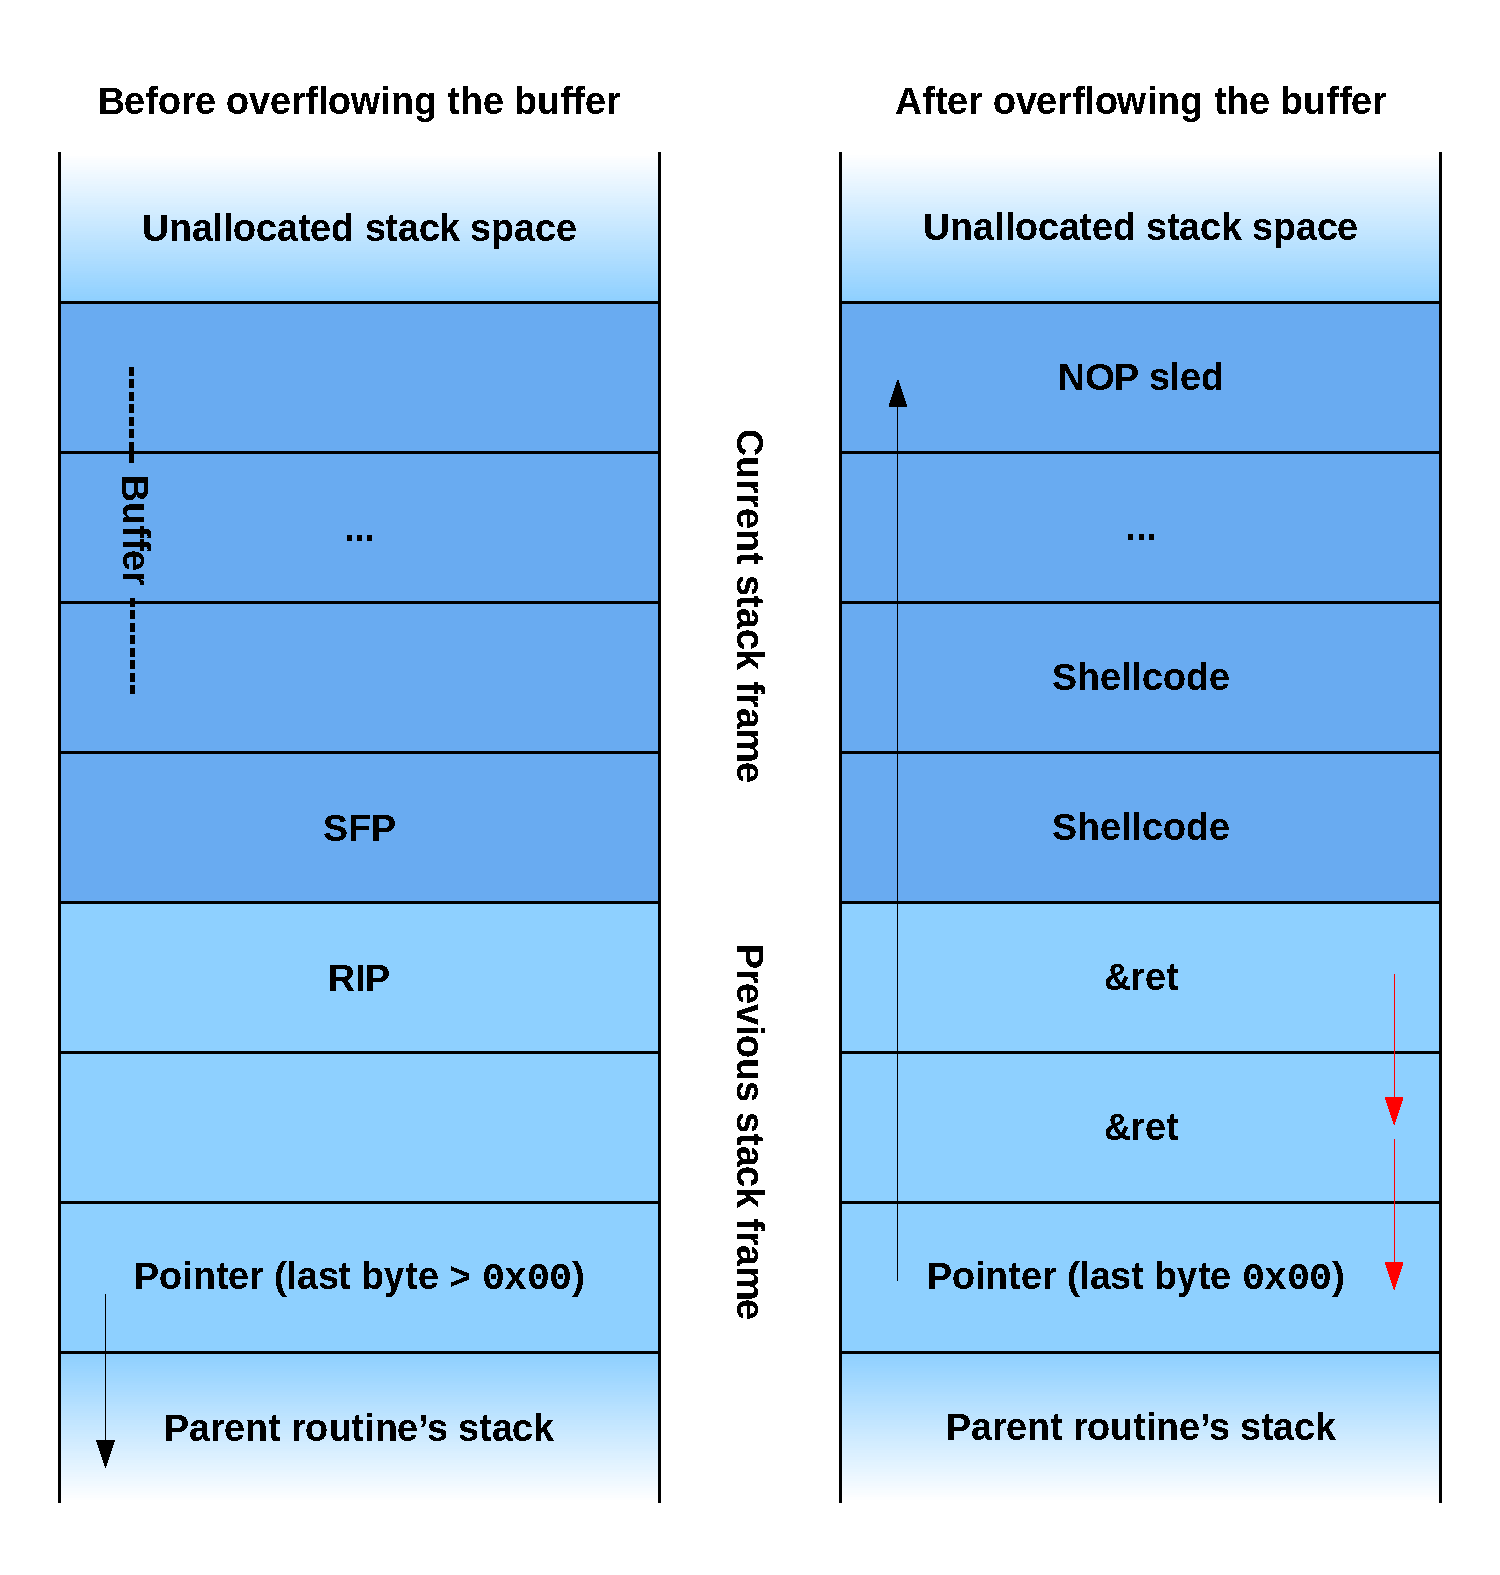
\includegraphics[width=0.7\textwidth]{figures/ret2ret}
	\caption{Stack layout before and after a stack buffer overflow with ret2ret approach (own graphical representation based on figure 16 in \cite[10]{Mueller2008})}
	\label{fig:ret2ret}
\end{figure}

\section*{ToDo}

\begin{itemize}
	\item{
		\gls{got} hijacking / overwriting (space constraints $\Rightarrow$ doesn't need as much space as shellcode or \gls{rop} chains) \cmark
	}
	\item{
		\gls{aslr} brute-force $\Rightarrow$ on \texttt{x86\_64} difficult because of too much entropy
	}
	\item{
		Return into non-radnomized memory (\gls{aslr} bypass) ret2text, ret2bss, ret2data: on non-\gls{pie}
	}
	\item{
		Pointer redirection: string or function pointers
	}
	\item{
		Integer overflows $\Rightarrow$ signedness or wrong width (e.g. \texttt{int} assignment to \texttt{char})
	}
	\item{
		Code injection: ret2esp, ret2ret, ret2pop, ret2eax
	}
	\item{
		Destructor overwriting ret2dtors
	}
	\item{
		Stack canaries: clone-probing to defeat canaries \textbf{and} \gls{aslr}
	}
\end{itemize}
